%%%%%%%%%%%%%%%%%%%%%%%%%%%%%%%%%%%%%%%%%
% Beamer Presentation
% LaTeX Template
% Version 1.0 (10/11/12)
%
% This template has been downloaded from:
% http://www.LaTeXTemplates.com
%
% License:
% CC BY-NC-SA 3.0 (http://creativecommons.org/licenses/by-nc-sa/3.0/)
%
%%%%%%%%%%%%%%%%%%%%%%%%%%%%%%%%%%%%%%%%%

%----------------------------------------------------------------------------------------
%	PACKAGES AND THEMES
%----------------------------------------------------------------------------------------

\documentclass{beamer}

\mode<presentation> {

% The Beamer class comes with a number of default slide themes
% which change the colors and layouts of slides. Below this is a list
% of all the themes, uncomment each in turn to see what they look like.

%\usetheme{default}
%\usetheme{AnnArbor}
%\usetheme{Antibes}
%\usetheme{Bergen}
%\usetheme{Berkeley}
%\usetheme{Berlin}
%\usetheme{Boadilla}
%\usetheme{CambridgeUS}
%\usetheme{Copenhagen}
%\usetheme{Darmstadt}
%\usetheme{Dresden}
%\usetheme{Frankfurt}
%\usetheme{Goettingen}
%\usetheme{Hannover}
%\usetheme{Ilmenau}
%\usetheme{JuanLesPins}
%\usetheme{Luebeck}
\usetheme{Madrid}
%\usetheme{Malmoe}
%\usetheme{Marburg}
%\usetheme{Montpellier}
%\usetheme{PaloAlto}
%\usetheme{Pittsburgh}
%\usetheme{Rochester}
%\usetheme{Singapore}
%\usetheme{Szeged}
%\usetheme{Warsaw}

% As well as themes, the Beamer class has a number of color themes
% for any slide theme. Uncomment each of these in turn to see how it
% changes the colors of your current slide theme.

%\usecolortheme{albatross}
%\usecolortheme{beaver}
%\usecolortheme{beetle}
%\usecolortheme{crane}
%\usecolortheme{dolphin}
%\usecolortheme{dove}
%\usecolortheme{fly}
%\usecolortheme{lily}
%\usecolortheme{orchid}
%\usecolortheme{rose}
%\usecolortheme{seagull}
%\usecolortheme{seahorse}
%\usecolortheme{whale}
%\usecolortheme{wolverine}

%\setbeamertemplate{footline} % To remove the footer line in all slides uncomment this line
%\setbeamertemplate{footline}[page number] % To replace the footer line in all slides with a simple slide count uncomment this line

%\setbeamertemplate{navigation symbols}{} % To remove the navigation symbols from the bottom of all slides uncomment this line
}

\usepackage[utf8]{inputenc}
\usepackage[portuguese]{babel}
\usepackage{color,soul}
\usepackage{graphicx} % Allows including images
\usepackage{booktabs} % Allows the use of \toprule, \midrule and \bottomrule in tables

%----------------------------------------------------------------------------------------
%	TITLE PAGE
%----------------------------------------------------------------------------------------

\title[Framework para Redes Sociais]{Framework para Redes Sociais baseadas em Compartilhamento de Rotas e Agendas}

\author{Álex Mesquita \& Jefferson Xavier}

\institute[UnB]
{
\textit{alex.mesquita0608@gmail.com}
\textit{jeffersonx.xavier@gmail.com}\\
Universidade de Brasília\\
\medskip
}
\date{01 de Julho de 2016}

\begin{document}

\begin{frame}
\titlepage
\begin{center}
Orientadores\\
Prof. Dr. Maurício Serrano\\
Prof. Dr. Milene Serrano
\end{center}
\end{frame}

\begin{frame}
\frametitle{Visão Geral}
\tableofcontents
\end{frame}

%----------------------------------------------------------------------------------------
%	PRESENTATION SLIDES
%----------------------------------------------------------------------------------------

\section{Questão de Pesquisa}

\begin{frame}
\frametitle{Questão de Pesquisa}

É possível oferecer um \textbf{\textit{framework}} que auxilie no desenvolvimento de redes sociais, disponibilizando recursos \textbf{específicos de definições de rotas e agenda} e recursos \textbf{gerais de relacionamentos}, proporcionando ao desenvolvedor facilidade ao lidar com preocupações intrínsecas desse contexto?

\begin{figure}[h]
	\centering
	
\includegraphics[scale=0.15]{figuras/search.eps}
\end{figure}

\end{frame}

\section{Justificativa}

\begin{frame}
\frametitle{Justificativa}

\begin{itemize}
	\item Crescimento de redes sociais virtuais;
	\item Falta de suporte para redes sociais com nichos específicos;
	\item Proporcionar desenvolvimento ágil e com maior qualidade.
\end{itemize}

\end{frame}


\section{Objetivos}
\subsection{Objetivo Geral}

\begin{frame}
\frametitle{Objetivo Geral}

Oferecer um \textit{framework} para ser utilizado no desenvolvimento de redes sociais, o qual disponibiliza recursos gerais de relacionamentos e específicos de definição de rotas e agenda, procurando auxiliar o desenvolvedor de software ao lidar com preocupações intrínsecas desse contexto.

\begin{figure}[h]
	\centering
	
\includegraphics[scale=0.4]{figuras/objective.eps}
\end{figure}

\end{frame}

\subsection{Objetivos Específicos}

\begin{frame}
\frametitle{Objetivos Específicos}

\begin{itemize}
	\item Definir uma arquitetura com base no \textbf{uso de grafos}, alinhada às boas práticas da Engenharia de Software, para representar os relacionamento entre as pessoas bem como as rotas percorridas por elas.
	\item Evoluir a arquitetura proposta, visando lidar com \textbf{algoritmos para compatibilizar agendas entre os interessados}.
\end{itemize}

\end{frame}

\begin{frame}
\frametitle{Objetivos Específicos}

\begin{itemize}
	\item \textbf{Usar estruturas de dados e algoritmos específicos}, visando \textbf{desempenho e facilidades na manutenção evolutiva do software}.
	\item \textbf{Instanciar um produto de software} - i.e. uma rede social específica - a partir do \textit{framework}, no intuito de coletar as primeiras impressões acerca do suporte desenvolvido como tema foco desse trabalho.
\end{itemize}

\end{frame}

\section{Proposta}

\begin{frame}
\frametitle{Proposta Apresentada}

\begin{itemize}
	\item Framework caixa cinza;
	\item Recursos de rotas;
	\item Recursos de agendas;
	\item Recursos gerais;
	\item Extensível, com pontos flexíveis;
	\item Tecnologia Ruby on Rails.
\end{itemize}

\begin{figure}[h]
	\centering
	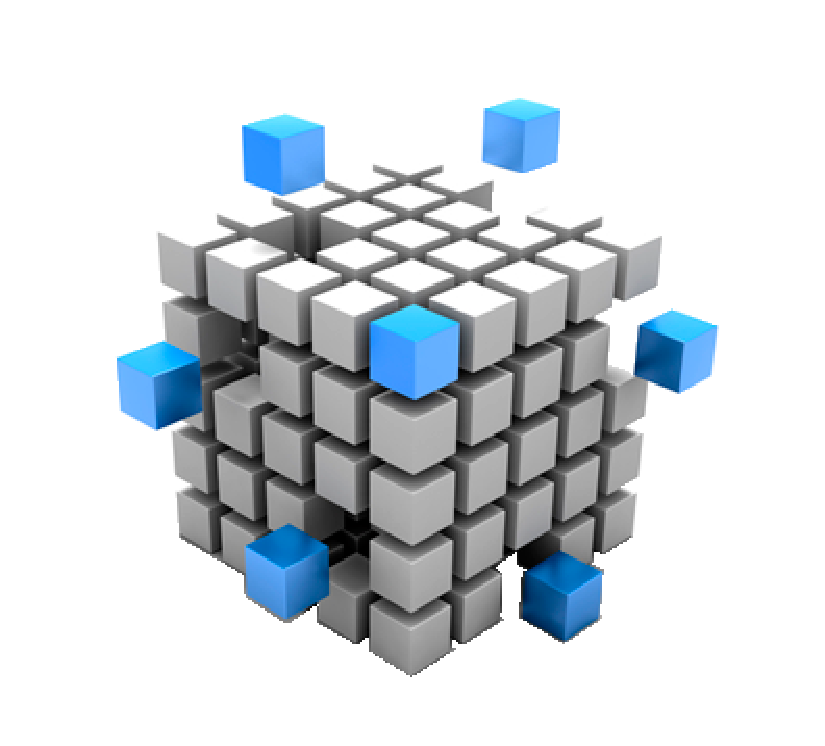
\includegraphics[scale=0.35]{figuras/framework.eps}
\end{figure}

\end{frame}

\begin{frame}
\frametitle{Uso do Framework}

\begin{figure}[!h]
	\centering
	\includegraphics[scale=0.45]{../figuras/proposta/uso_proposto.eps}
	\caption{Modelo ilustrando um possível uso do \textit{Framework}}
	\label{uso_proposto}
\end{figure}

\end{frame}

\section{SocialFramework}

\begin{frame}
\frametitle{SocialFramework - Primeiros Passos}

\begin{itemize}
	\item Publicado oficialmente no RubyGems versão 1.0.1;
	\item gem `social\_framework';
	\item Arquivos de configuração:
	\begin{itemize}
		\item devise.rb
		\item social\_framework.rb
	\end{itemize}
\end{itemize}

\end{frame}

\begin{frame}
\frametitle{Scripts de Geração}

\begin{itemize}
	\item Arquivos de configuração: rails generate social\_framework:install;
	\item \textit{Models}: \textit{User}, \textit{Edge}, \textit{Schedule}, \textit{Event}, \textit{ParticipantEvent}, \textit{Route}, \textit{Location};
	\item \textit{Controllers} do plugin `Devise';
	\item \textit{Views} do plugin `Devise';
\end{itemize}

\end{frame}

\begin{frame}
\frametitle{Módulo de Usuários}

\begin{itemize}
	\item Recursos gerais de redes sociais;
	\item Uso do plugin `Devise':
	\begin{itemize}
		\item Registros;
		\item Autenticações;
		\item Validações;
	\end{itemize}
	\item Relacionamentos;
	\item Pesquisas;
	\item Sugestão de relacionamentos.
\end{itemize}

\end{frame}

\begin{frame}
\frametitle{Módulo de Usuários - Estrutura}

\begin{itemize}
	\item Classes de modelo \textit{User} e \textit{Edge};
	\item Muitos relacionamentos;
	\begin{itemize}
		\item Bidirecionais;
		\item Unidirecionais;
		\item Muitos tipos;
		\item Uma aresta para cada tipo de relacionamento;
	\end{itemize}
	\item Grafo construído até uma profundidade pré-estabelecida (Usuários e Eventos);
	\item Sugestão de amizades considerando o terceiro nível do grafo com algoritmo DFS;
	\item Pesquisas realizadas no grafo com o algoritmo BFS e em banco de dados;
\end{itemize}

\end{frame}

\begin{frame}
\frametitle{Módulo de Agenda}

\begin{itemize}
	\item Conciliação de horários;
	\item Marcação de eventos;
	\item Uma agenda para cada usuário;
	\item Classes de modelo \textit{Schedule}, \textit{Event} e \textit{ParticipantEvent}.
\end{itemize}

\end{frame}

\begin{frame}
\frametitle{Conciliação de Horários}

\begin{itemize}
	\item Grupos de usuários;
	\item Período maior pré-definido (Uma semana);
	\item Período diário pré-definido (De 08:00hs às 18:00hs);
	\item Duração de \textit{Slots} pré-definida (Uma hora).
\end{itemize}

\end{frame}

\begin{frame}
\frametitle{Conciliação de Horários - Estrutura}

\begin{itemize}
	\item Grafo bipartido;
	\item Vértices de slots e usuários;
	\item Pesos para usuários;
	\item Usuários fixos;
\end{itemize}

\begin{figure}[h]
	\centering
	\includegraphics[scale=0.35]{figuras/melhor_horario.eps}
	\caption{Grafo bipartido para procura do melhor horário}
\end{figure}

\end{frame}

\begin{frame}
\frametitle{Módulo de Rotas}

\begin{itemize}
	\item Definição de muitas rotas para muitos usuários;
	\item Mesma rota para múltiplos usuários;
	\item Comparação de rotas;
	\item Google Maps API;
	\begin{itemize}
		\item Requisições de pontos de Latitude e Longitude;
		\item Tipos de rotas: Carro, A Pé, Bicicleta ou Transporte público.
	\end{itemize}
\end{itemize}

\end{frame}

\begin{frame}
\frametitle{Comparação de Rotas}

\begin{itemize}
	\item Rota principal e rota secundária;
	\item Uso de desvio aceito definido para cada rota;
	\item Alteração da rota principal para atender a rota secundária e vice-versa;
	\item Algoritmo para buscar a melhor opção para a rota secundária;
	\item Informações de compatibilidade, pontos de mudanças e distância.
\end{itemize}

\end{frame}

\begin{frame}
\frametitle{Comparação de Rotas}

\begin{figure}[h]
	\centering
	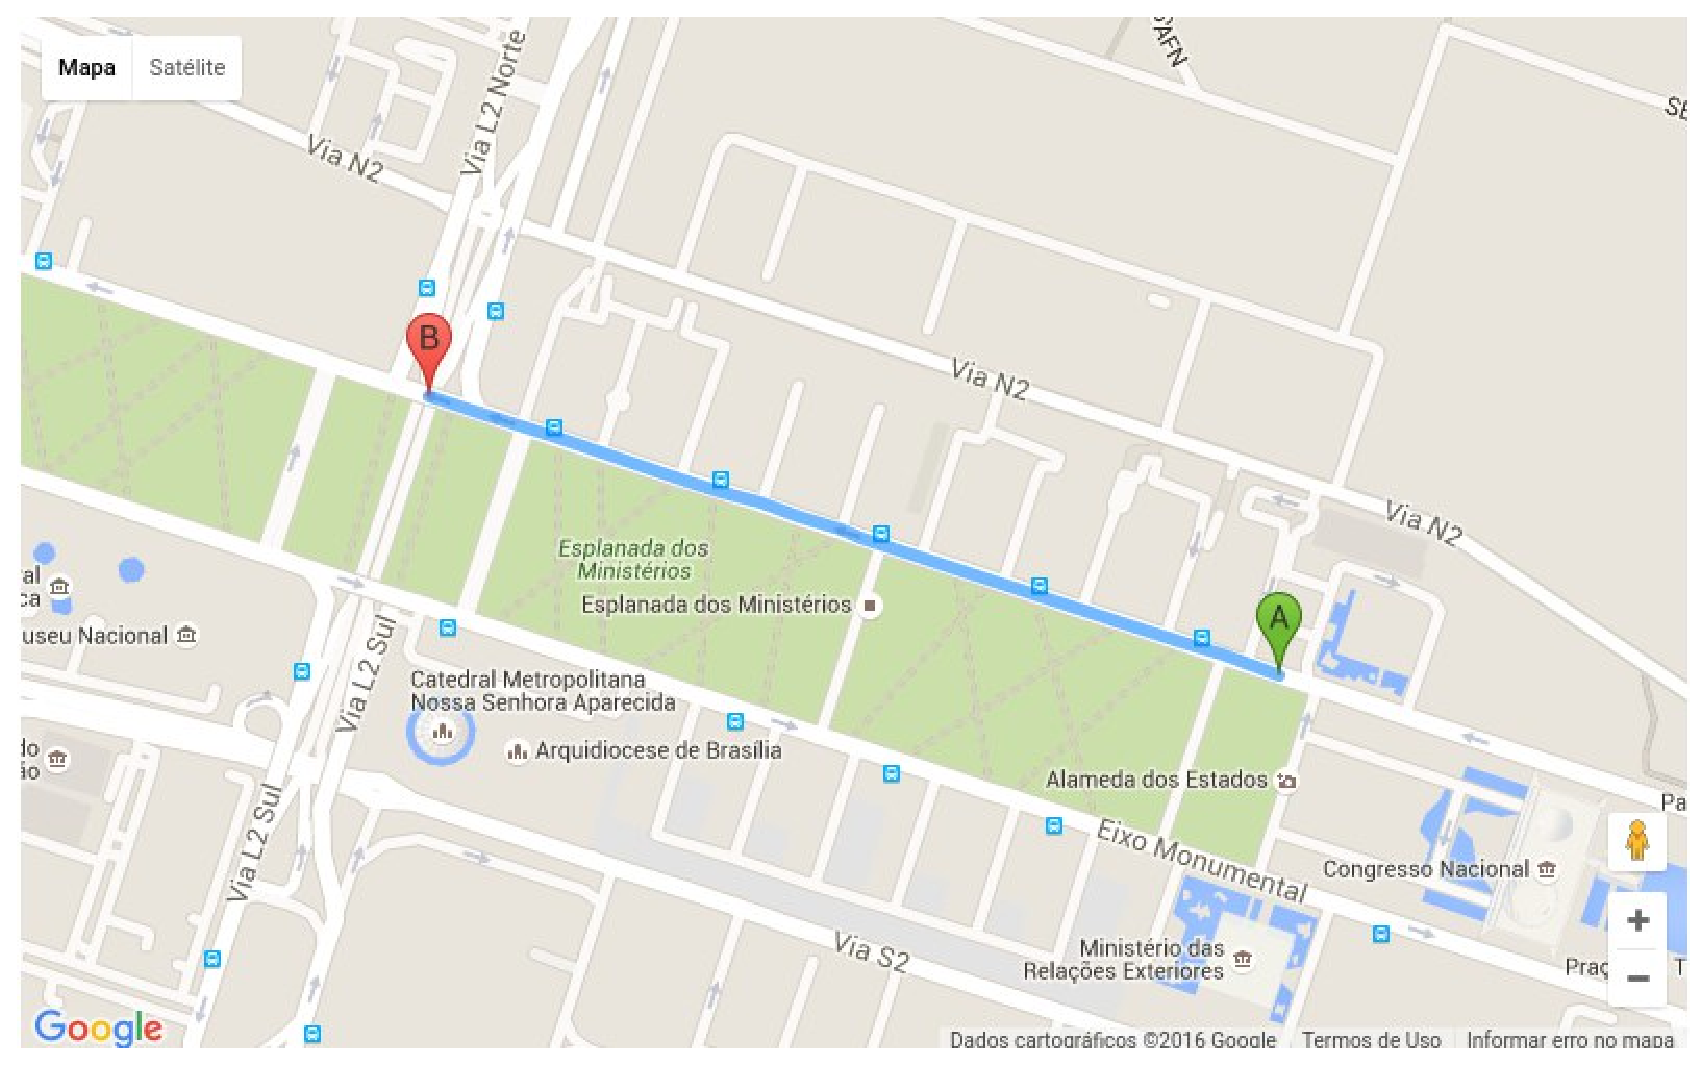
\includegraphics[scale=0.35]{figuras/rota1.eps}
	\caption{Rota principal original}
\end{figure}

\end{frame}

\begin{frame}
\frametitle{Comparação de Rotas}

\begin{figure}[h]
	\centering
	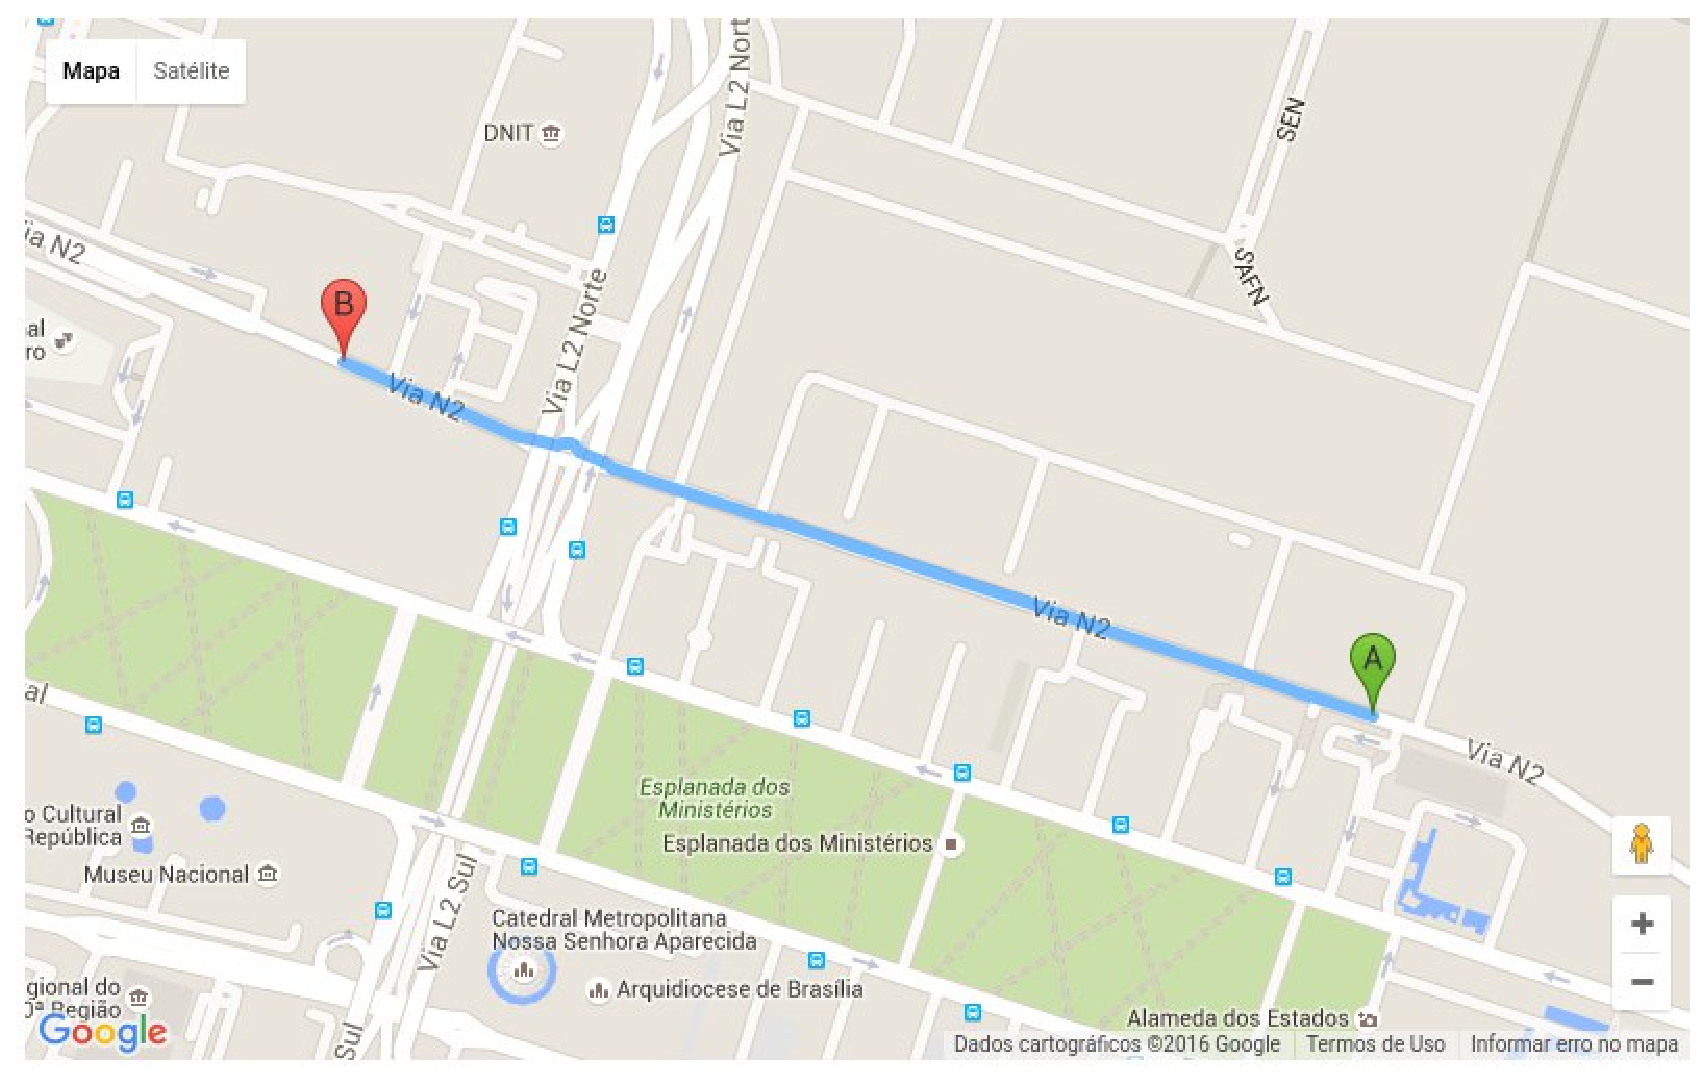
\includegraphics[scale=0.35]{figuras/rota2.eps}
	\caption{Rota secundária original}
\end{figure}

\end{frame}

\begin{frame}
\frametitle{Comparação de Rotas}

\begin{figure}[h]
	\centering
	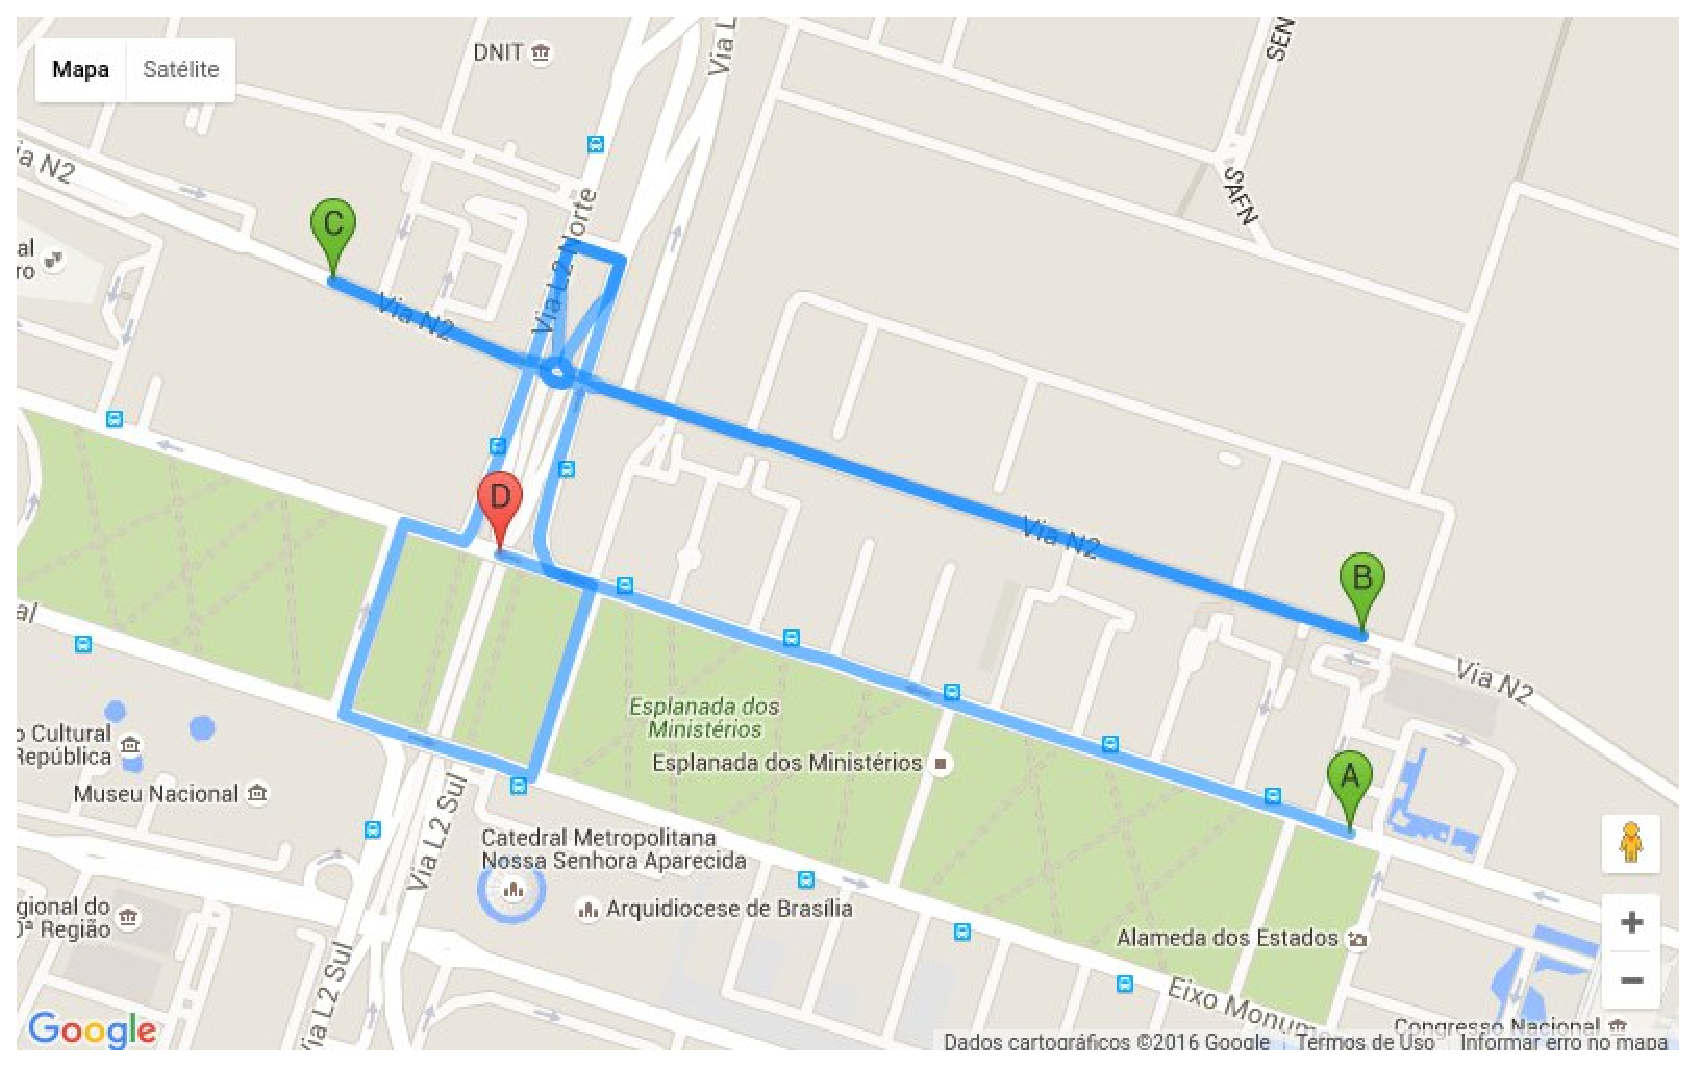
\includegraphics[scale=0.35]{figuras/juncao_rotas.eps}
	\caption{Rota principal final passando pela origem e destino da rota secundária}
\end{figure}

\end{frame}

\begin{frame}
\frametitle{Comparação de Rotas}

\begin{itemize}
	\item Rotas podem ser alteradas em ambos os pontos de origem e destino, apenas em algum deles, apenas na origem, apenas no destino ou em nenhum ponto.
	\item No caso de não ser possível alterar a rota principal, a rota secundária deve poder ser alterada;
	\item Caso a rota secundária não possa ser alterada as rotas são incompatíveis.
\end{itemize}

\end{frame}

\begin{frame}
\frametitle{Hotspots}

\begin{itemize}
	\item Pontos de flexibilidade do framework;
	\item Framework todo extensível;
	\item Três padrões implementados: \textit{Factory Method}, \textit{Abstract Factory} e \textit{Strategy}.
\end{itemize}

\end{frame}

\begin{frame}
\frametitle{Hotspots - Factory Method}

\begin{itemize}
	\item Adaptação do padrão utilizada;
	\item Usado para as classes de modelo;
	\item Nomes das classes de modelo definidas no arquivo de configurações `social\_framework.rb';
\end{itemize}

\begin{figure}[h]
	\centering
	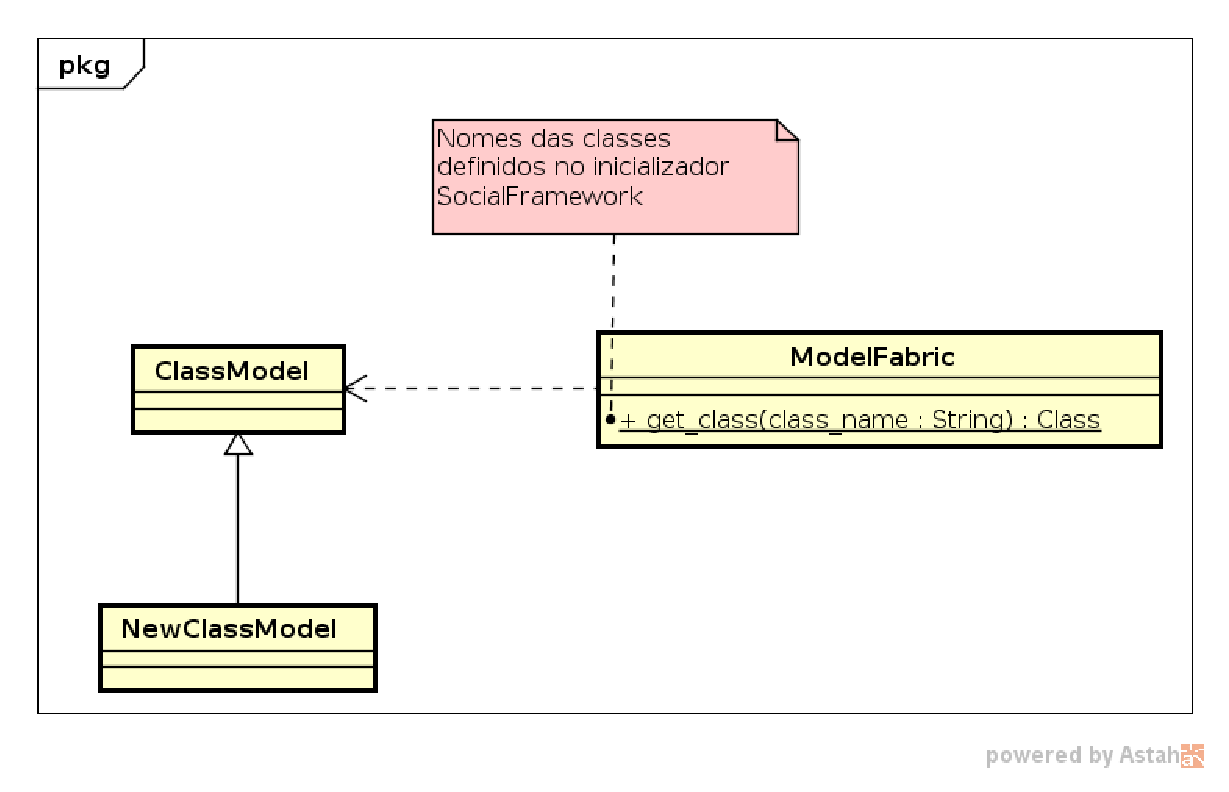
\includegraphics[scale=0.35]{figuras/factory_method.eps}
	\caption{Modelo do Factory Method}
\end{figure}

\end{frame}

\begin{frame}
\frametitle{Hotspots - Abstract Factory}

\begin{itemize}
	\item Usado para os elementos dos grafos (Vértices e Arestas);
	\item Classes com comportamento padrão implementadas;
\end{itemize}

\begin{figure}[h]
	\centering
	\includegraphics[scale=0.25]{figuras/abstract_factory.eps}
	\caption{Modelo do Abstract Factory}
\end{figure}

\end{frame}

\begin{frame}
\frametitle{Hotspots - Strategy}

\begin{itemize}
	\item Usado para cada um dos módulos do SocialFramework.
\end{itemize}

\begin{figure}[h]
	\centering
	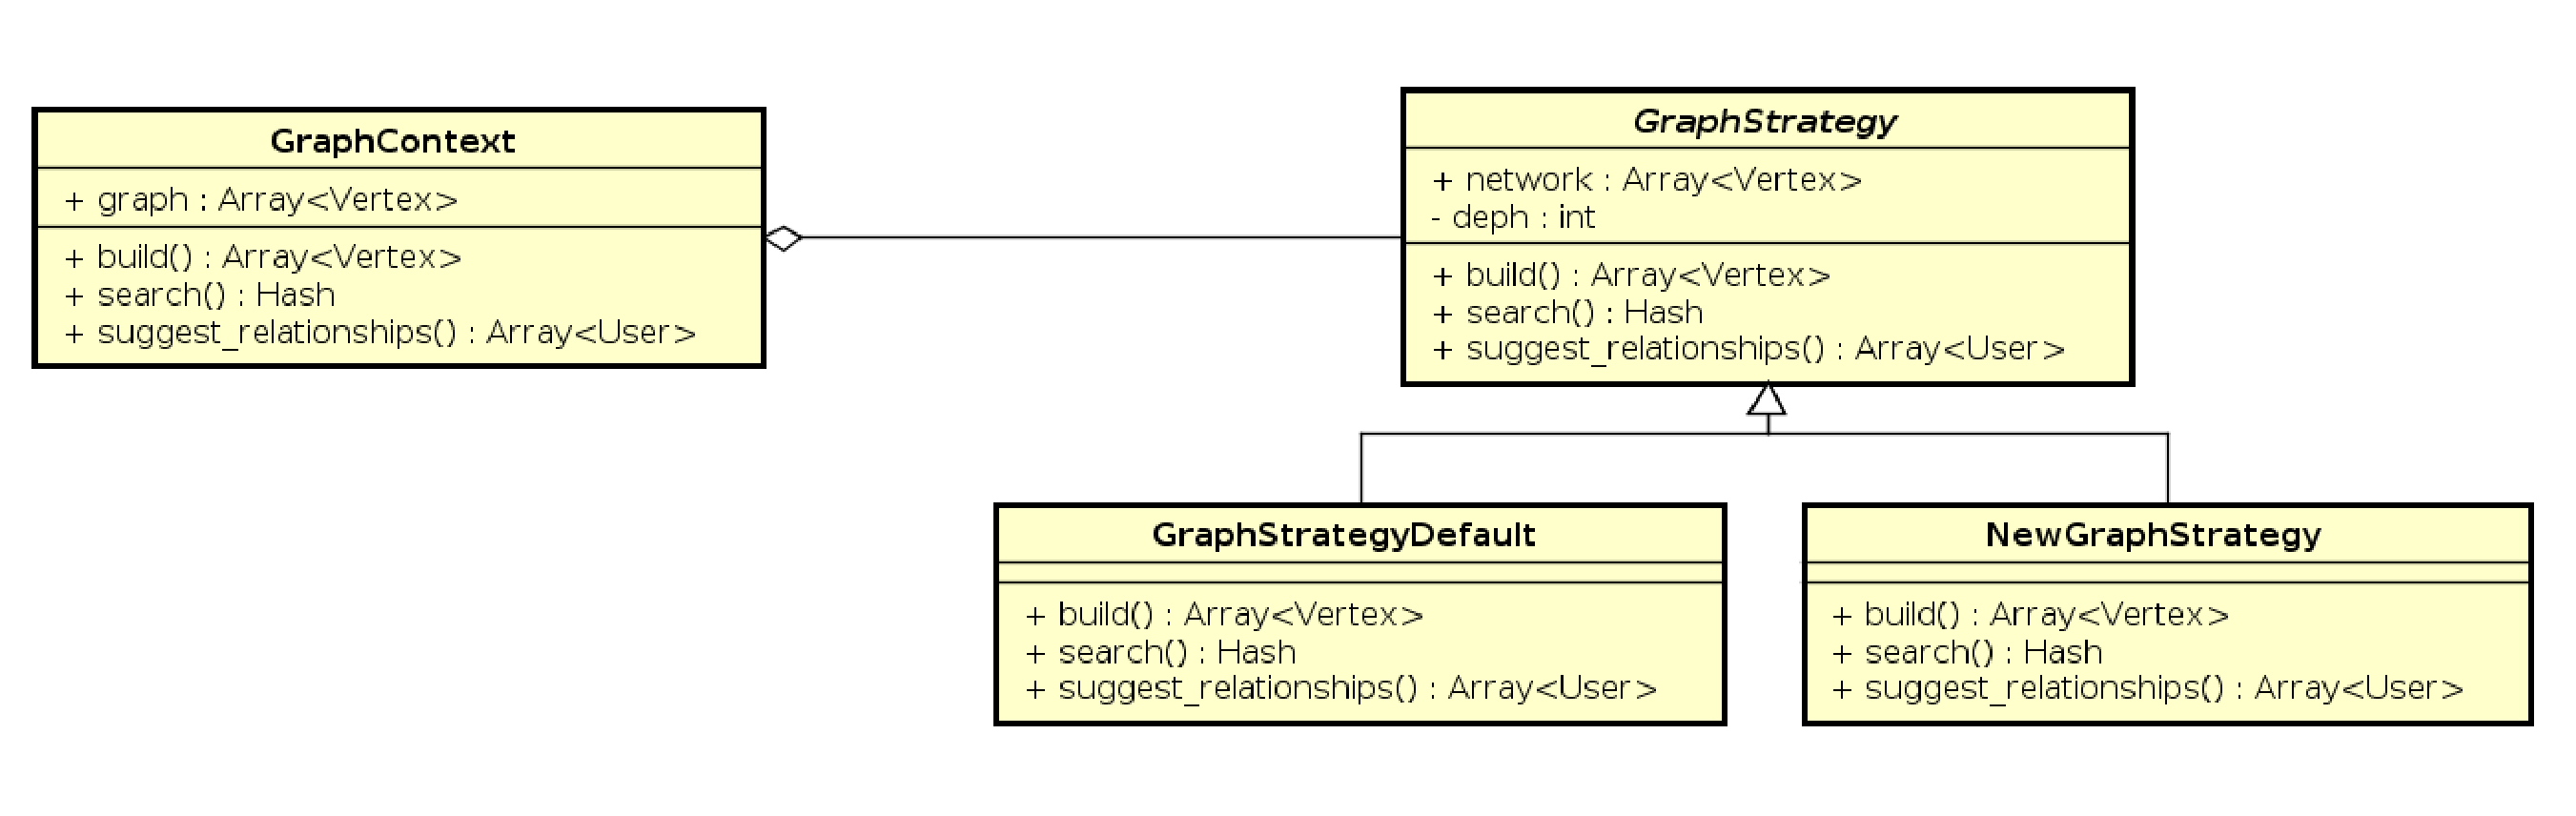
\includegraphics[scale=0.25]{figuras/graph_strategy.eps}
	\caption{Modelo do Strategy para o módulo de usuários}
\end{figure}

\end{frame}

\begin{frame}
\frametitle{Hotspots - Strategy}

\begin{figure}[h]
	\centering
	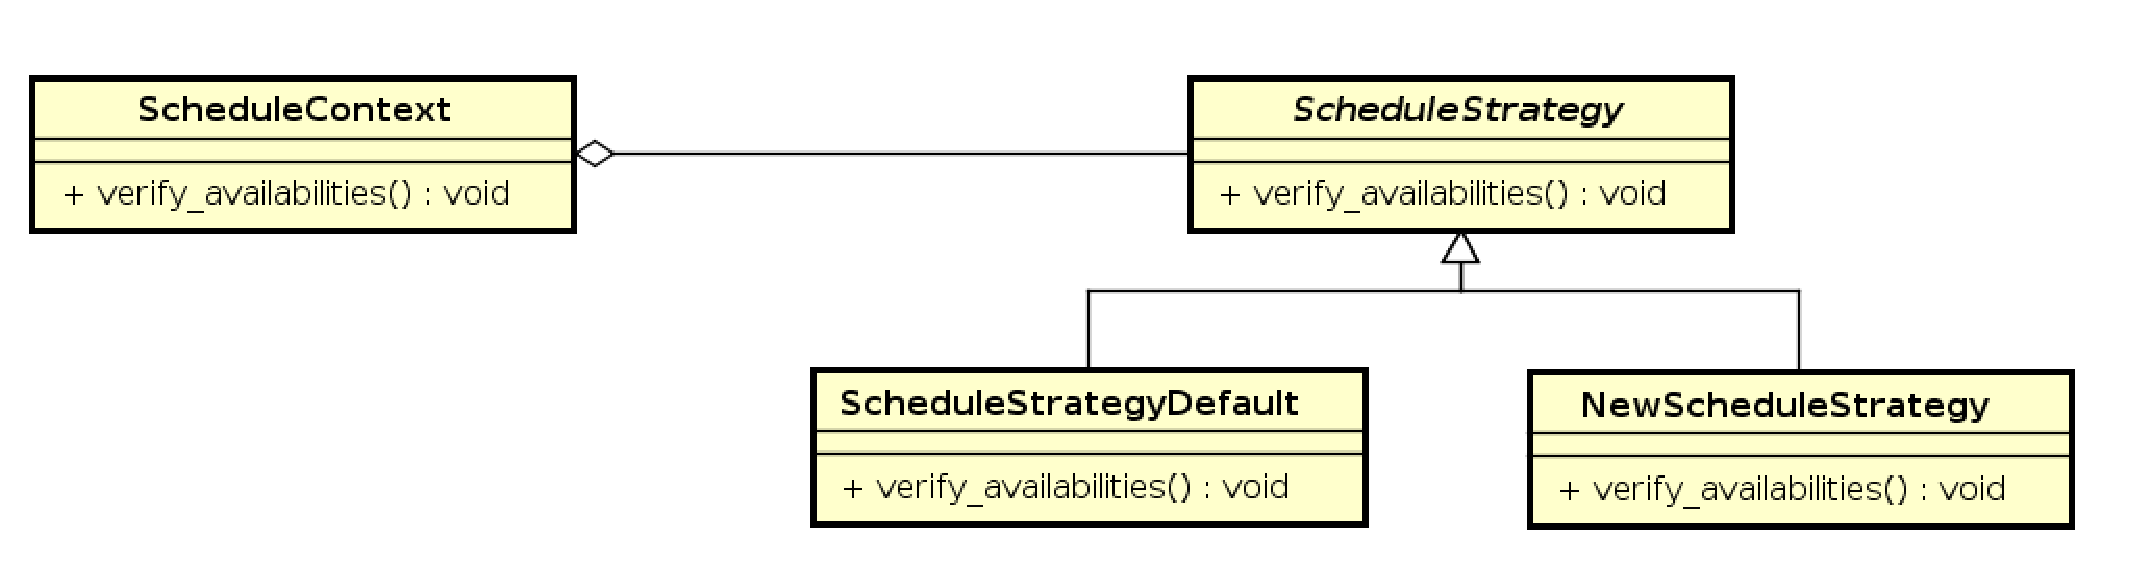
\includegraphics[scale=0.25]{figuras/schedule_strategy.eps}
	\caption{Modelo do Strategy para o módulo de agenda}
\end{figure}

\begin{figure}[h]
	\centering
	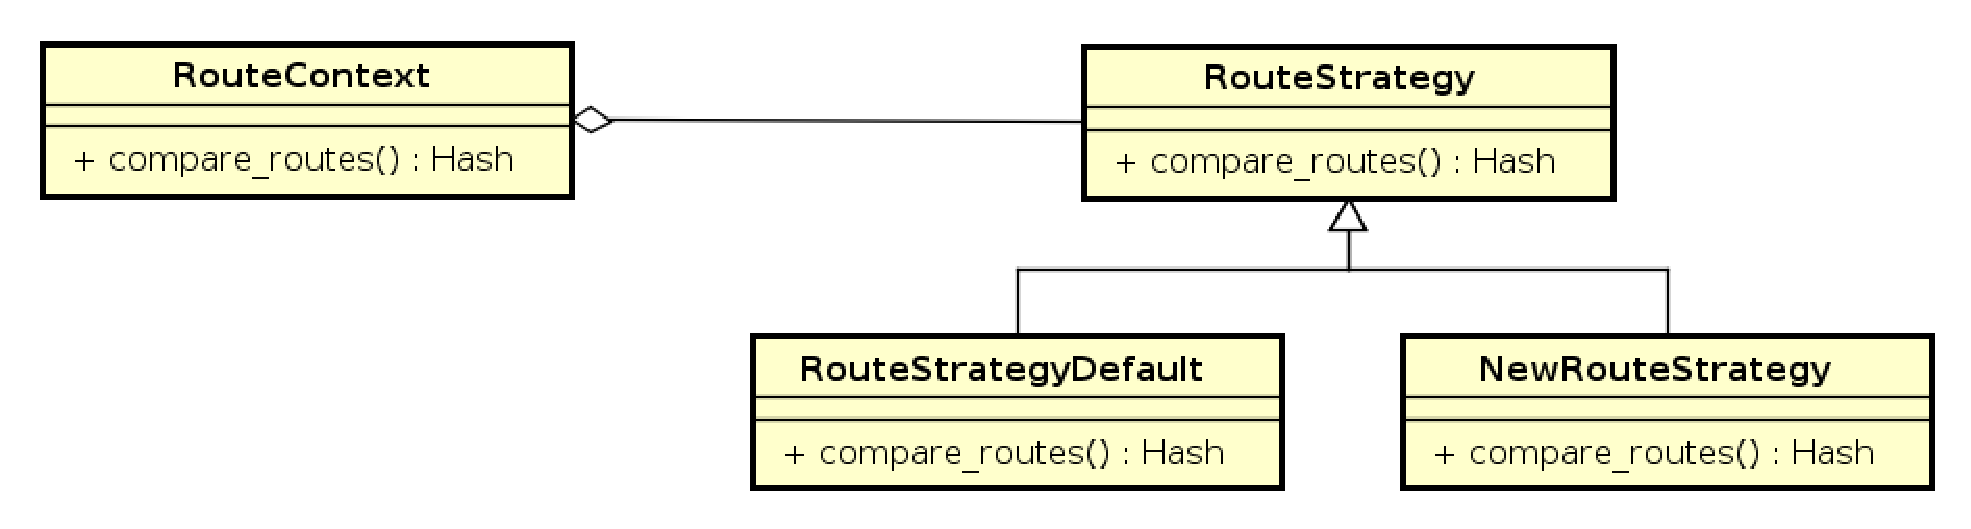
\includegraphics[scale=0.25]{figuras/route_strategy.eps}
	\caption{Modelo do Strategy para o módulo de rotas}
\end{figure}

\end{frame}

\section{Resultados}

\begin{frame}
\frametitle{Testes Unitários}

\begin{figure}[h]
	\centering
	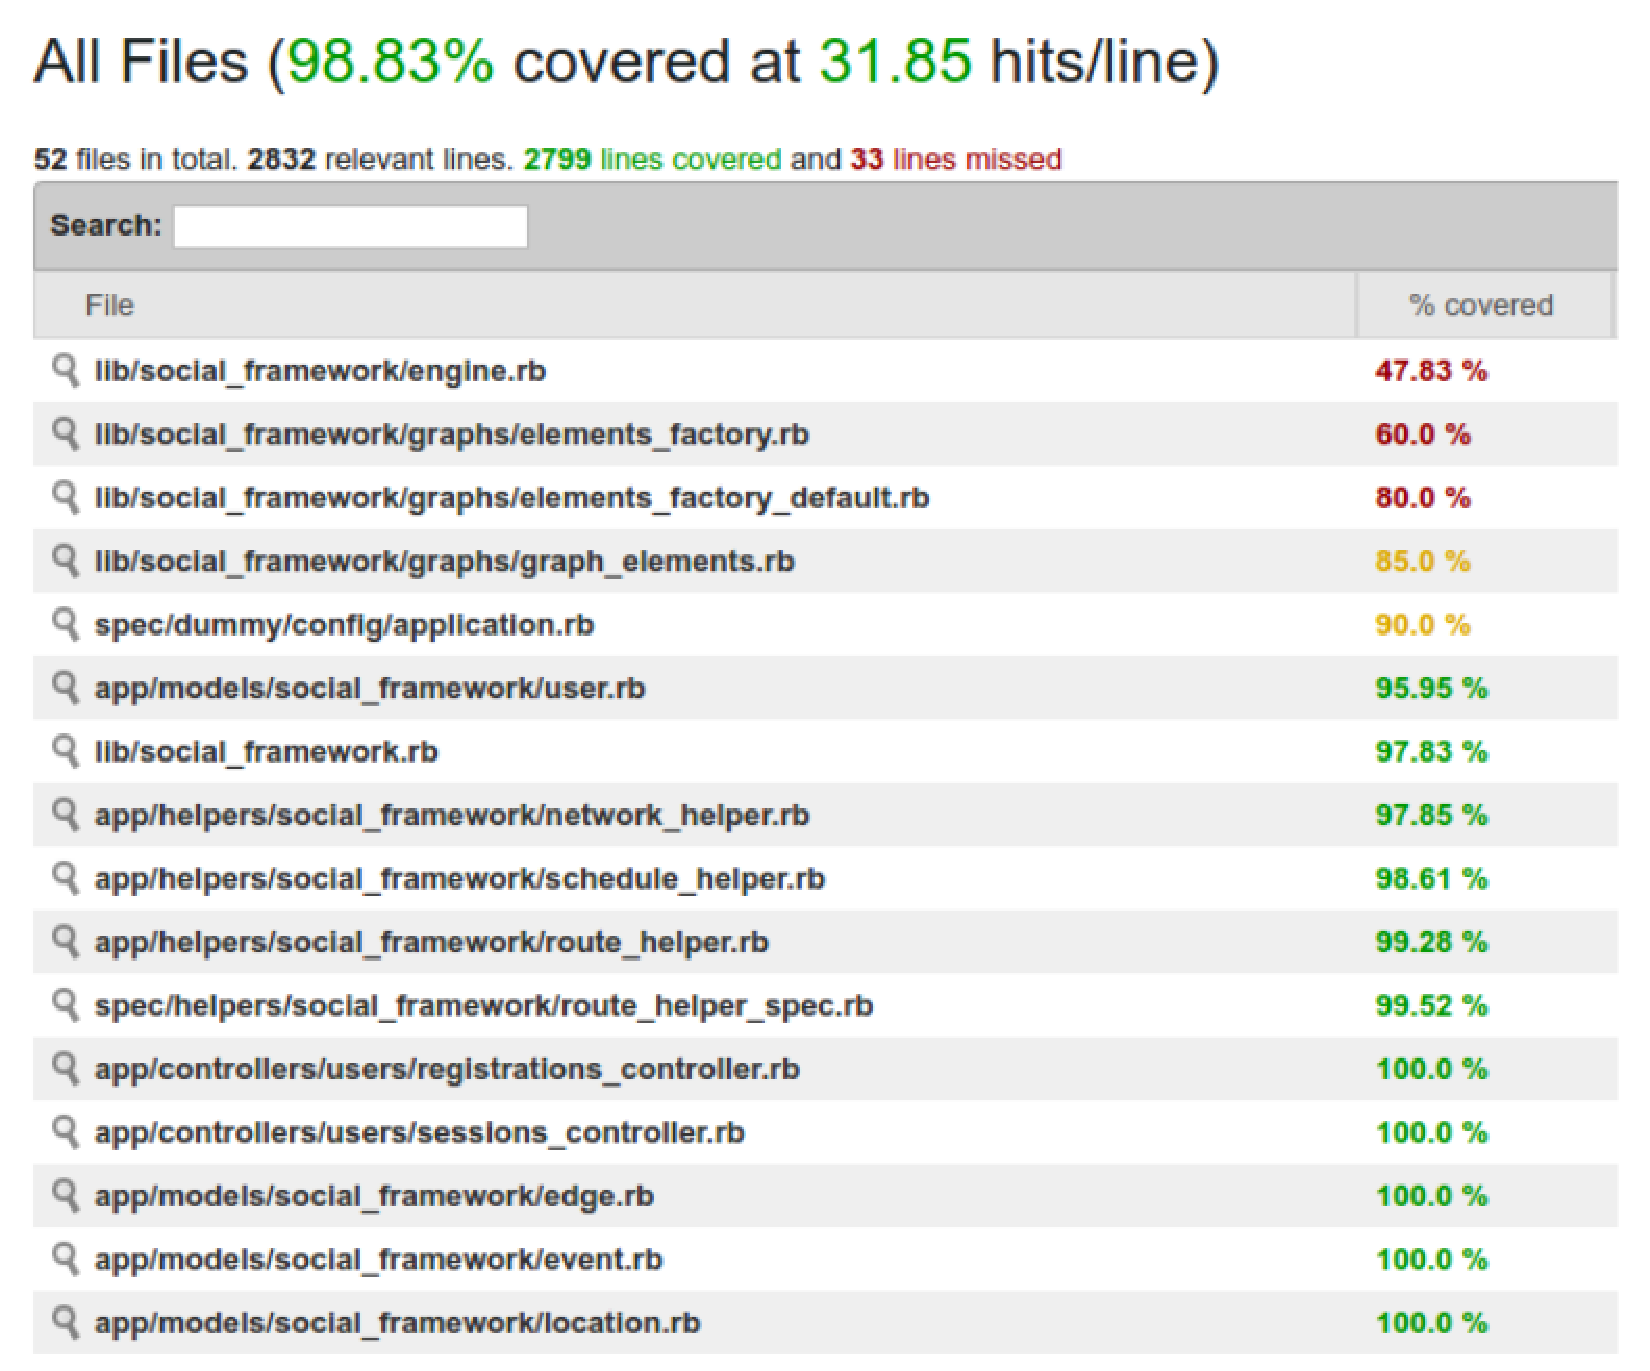
\includegraphics[scale=0.35]{figuras/cobertura.eps}
\end{figure}

\end{frame}

\begin{frame}
\frametitle{Desempenho}

\begin{itemize}
	\item{Construção}
\end{itemize}

\begin{figure}[h]
	\centering
	\includegraphics[scale=0.215]{figuras/desempenho/construcao.eps}
\end{figure}

\end{frame}

\begin{frame}
\frametitle{Desempenho}

\begin{itemize}
	\item{Pesquisas}
\end{itemize}

\begin{figure}[h]
	\centering
	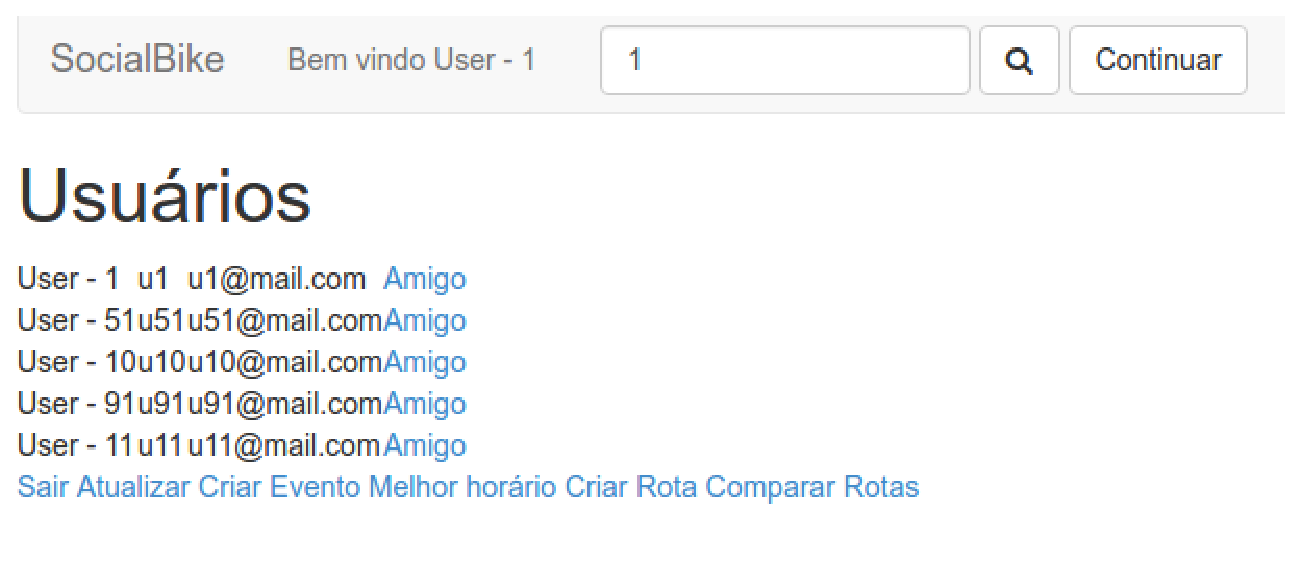
\includegraphics[scale=0.215]{figuras/desempenho/pesquisa.eps}
\end{figure}

\end{frame}

\begin{frame}
\frametitle{Desempenho}

\begin{itemize}
	\item{Sugestão de Relacionamentos}
\end{itemize}

\begin{figure}[h]
	\centering
	\includegraphics[scale=0.35]{figuras/desempenho/sugestao_relacionamentos.eps}
\end{figure}

\end{frame}

\begin{frame}
\frametitle{Desempenho}

\begin{itemize}
	\item{Sugestão de horário com tempo fixo}
\end{itemize}

\begin{figure}[h]
	\centering
	\includegraphics[scale=0.215]{figuras/desempenho/31_dias.eps}
\end{figure}

\end{frame}

\begin{frame}
\frametitle{Desempenho}

\begin{itemize}
	\item{Sugestão de horário com usuários fixos}
\end{itemize}

\begin{figure}[h]
	\centering
	\includegraphics[scale=0.215]{figuras/desempenho/500_users.eps}
\end{figure}

\end{frame}

\begin{frame}
\frametitle{Qualidade do Código}

\begin{figure}[!h]
	\centering
	\includegraphics[scale=0.5]{figuras/gpa.eps}
\end{figure}

\begin{itemize}
	\item{Quantidade de arquivos com cada nota:}
\end{itemize}

\begin{table}[!h]
\centering
\begin{tabular}{cccccc}
\toprule
\textbf{Nota A} & \textbf{Nota B} & \textbf{Nota C} & \textbf{Nota D} & \textbf{Nota E} & \textbf{Nota F} \\ \midrule
50 & 2 & 1 & 0 & 0 & 0							   \\ \bottomrule
\end{tabular}
\end{table}

\end{frame}

\begin{frame}
\Huge{\centerline{Obrigado!}}
\end{frame}

\begin{frame}
\frametitle{Referências}
\footnotesize{
\begin{thebibliography}{99} % Beamer does not support BibTeX so references must be inserted manually as below
\bibitem[Krueger, 1992]{krueger} Krueger, Charles W. (1992)
\newblock Software Reuse
\bibitem[Marteleto, 2001]{marteleto} Marteleto, Regina Maria (2001)
\newblock Mídias Sociais: uma contribuição de análise
\end{thebibliography}
}
\end{frame}

\end{document} 